%%%%%%%%%%%%%%%%%%%%%%%%%%%%%%%%%%%%%%%%%%%%%%%%%%%%%%%%%%%%%%%%%%%%%%%%%%%%%%%%
% Author : Petr Balcar, Tomas Polasek (template)
% Description : Seventh exercise in the Introduction to Game Development course.
%   It deals with the creation of a Game Design Document, presenting a short 
%   pitch for a potential game project.
%%%%%%%%%%%%%%%%%%%%%%%%%%%%%%%%%%%%%%%%%%%%%%%%%%%%%%%%%%%%%%%%%%%%%%%%%%%%%%%%

\documentclass[a4paper,10pt,english]{article}

\usepackage[left=2.50cm,right=2.50cm,top=1.50cm,bottom=2.50cm]{geometry}
\usepackage[utf8]{inputenc}

% Hyper-Text References
\usepackage{hyperref}
\hypersetup{colorlinks=true, urlcolor=blue}

% Drawing Images and Graphs
\usepackage{tikz}
\usepackage{pgfplots}

% Page Utilities
\usepackage{graphicx}

% Image Sub-Captions
\usepackage{subcaption}

\newcommand{\ph}[1]{\textit{[#1]}}

\title{%
Game Pitch Document%
}
\author{%
Petr Balcar (xbalca11)%
}
\date{}

\begin{document}

\maketitle
\thispagestyle{empty}

{%
\large

\begin{itemize}

\item[] \textbf{Title:} Stranded and Augmented

\item[] \textbf{Genre:} Rouge-like

\item[] \textbf{Style:} Futuristic, Intergalactic, Cybernetic

\item[] \textbf{Platform:} Windows, Mobile

\item[] \textbf{Market:} Newbie/casual gamer, aged 16+

\item[] \textbf{Elevator Pitch:} A game, where \emph{health} is \emph{wealth}. How much of yourself are willing to give up to return home?

\end{itemize}

}

\section*{\centering The Pitch}

\subsection*{Introduction}
A unique rogue-like, where health is money. Saving your augmentations and equipment against weak enemies is most likely the best bet, but be careful to judge, because the consequences can be deadly...
Fight enemies, sell and buy upgrades, but most importantly rebuild your ship so you can get back home.

\subsection*{Background}
Getting a powerful setup using various upgrades and combos is an incredibly fun part of many rogue-like games, such as \emph{Slay the Spire} or \emph{Hades}. 

This idea is expanded upon, and in a similar style to \emph{Balatro}, where players try to play just the right hand to clear a level, \emph{Stranded and Augmented} makes you risk yourself to gain more rewards.

\subsection*{Setting}
Your ship crashes on a lonely planet. Only you and bits of the ship remain. So this is where it ends...
Luckily, the planet is not as abandoned as you first thought. Everyone here is so welcoming and helpful.
Is it their nature? Or are they just interested in your biomechanical augmentations? Or perhaps you are yet to meet \emph{everyone}.

You scour the planet in search of the lost pieces of the ship while defeating enemies, selling your augmentations, and buying new ones while just barely staying \emph{alive}.

\subsection*{Features}
\emph{Stranded and Augmented} will include features like:

\begin{itemize}
    \item Basic economy - so selling some of your gear is a worthy investment
    \item Smooth combat with various enemies
    \item Unique boss fights, where upgrades will be essential
    \item Synergistic upgrades
    \item Shops with upgrades, augmentations, etc.
    \item A reactive story
\end{itemize}

\subsection*{Genre}
A rogue-like with a compelling story and a twist that makes you risk.

\subsection*{Platform}
\emph{Stranded and Augmented} will be released first on Windows and potentially adapted to mobile.

\subsection*{Style}
\emph{Stranded and Augmented} has a serious, futuristic, cybernetic style that allows for interesting characters and jaw-dropping landscapes.

\begin{figure}[h]
    \centering
    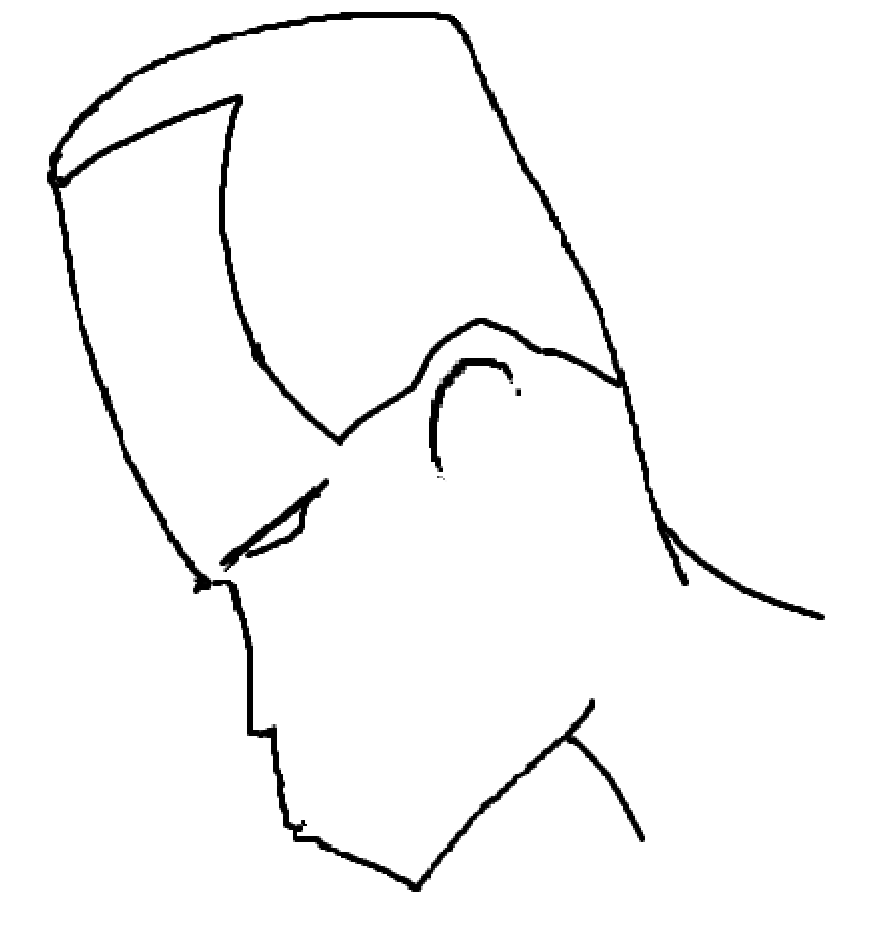
\includegraphics[width=0.25\linewidth]{StrandedAndAugmentedProtagonist.png}
    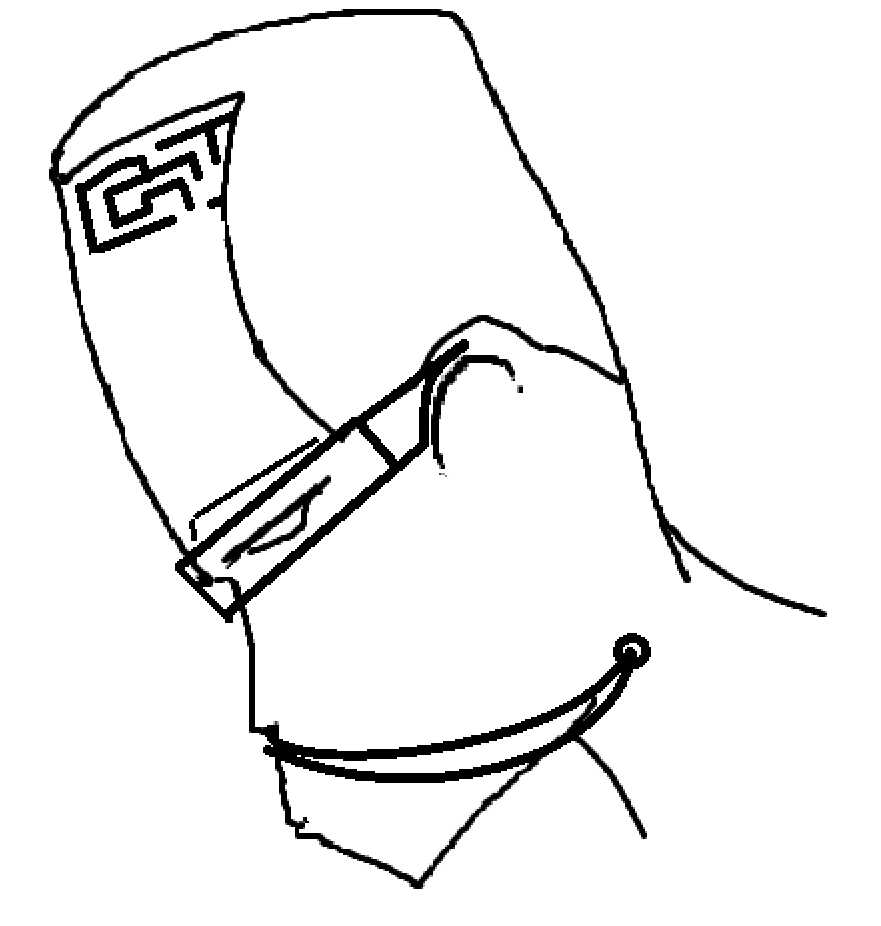
\includegraphics[width=0.25\linewidth]{StrandedAndAugmentedProtagonistAugmented.png}
    \caption{Concept art of the protagonist's face, without and with augmentations}
\end{figure}

\begin{figure}[h]
    \centering
    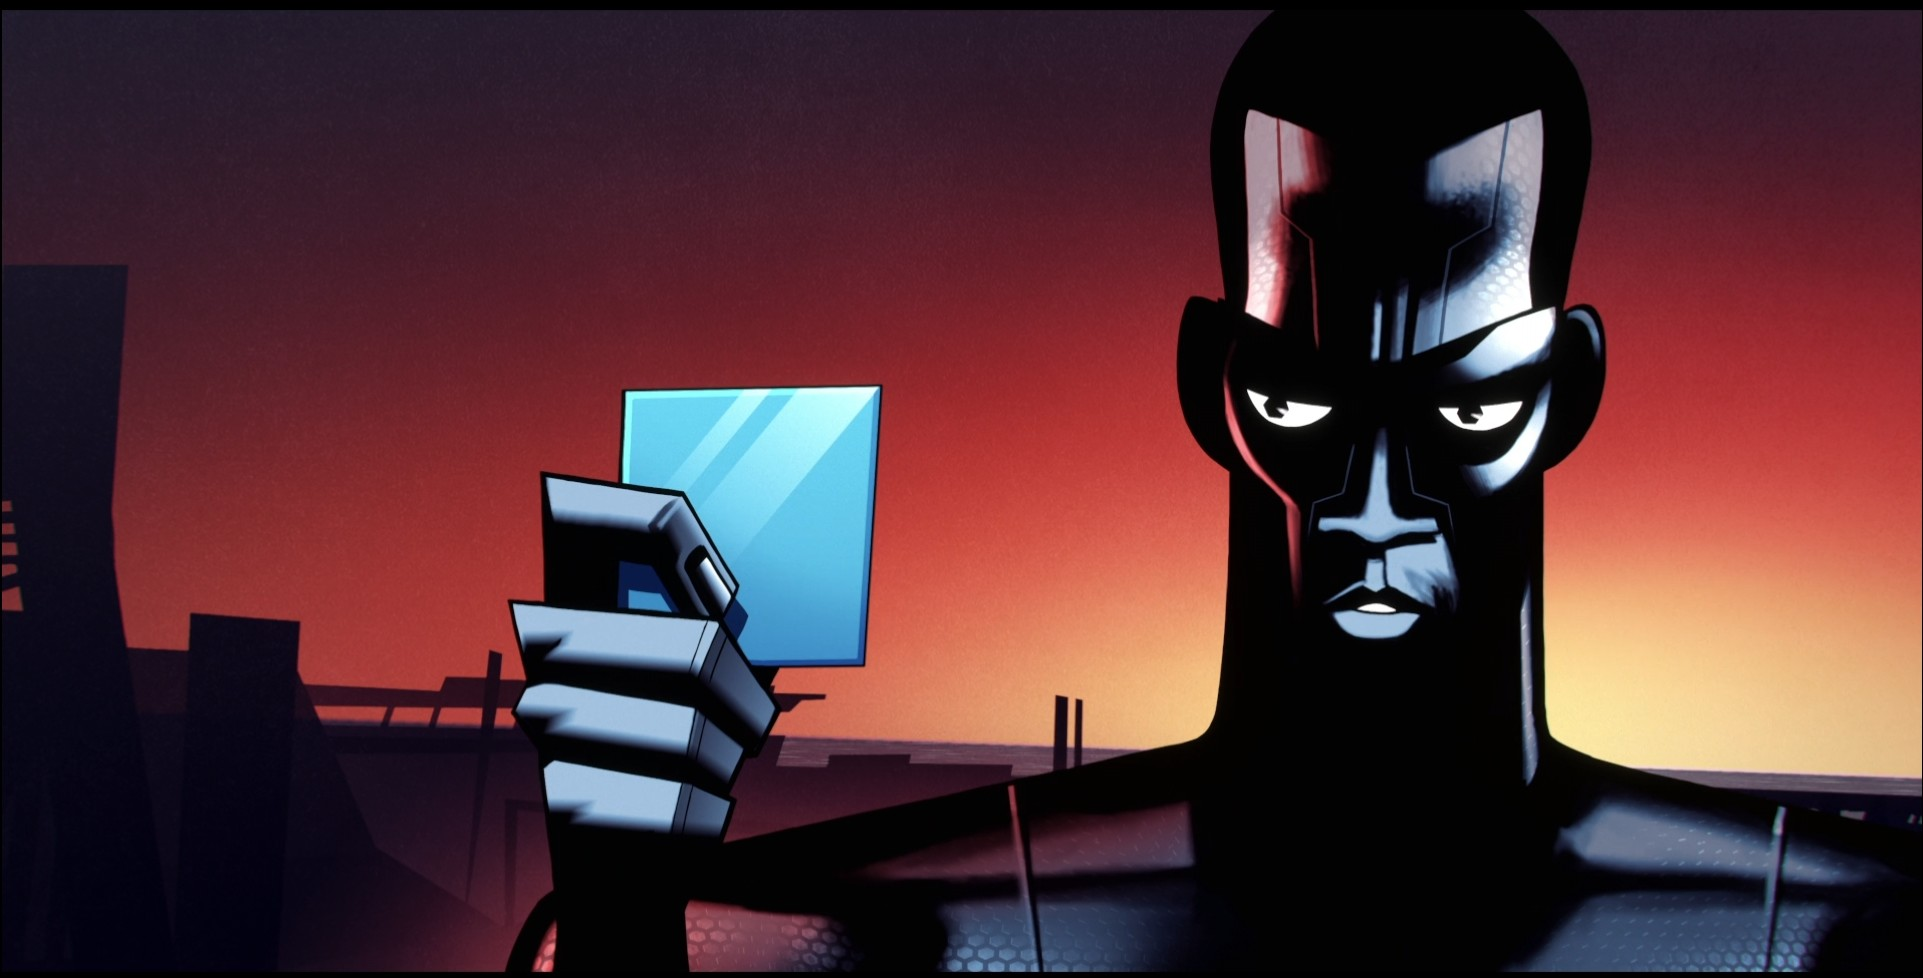
\includegraphics[width=0.6\linewidth]{LoveDeathAndRobotsZima.jpg}
    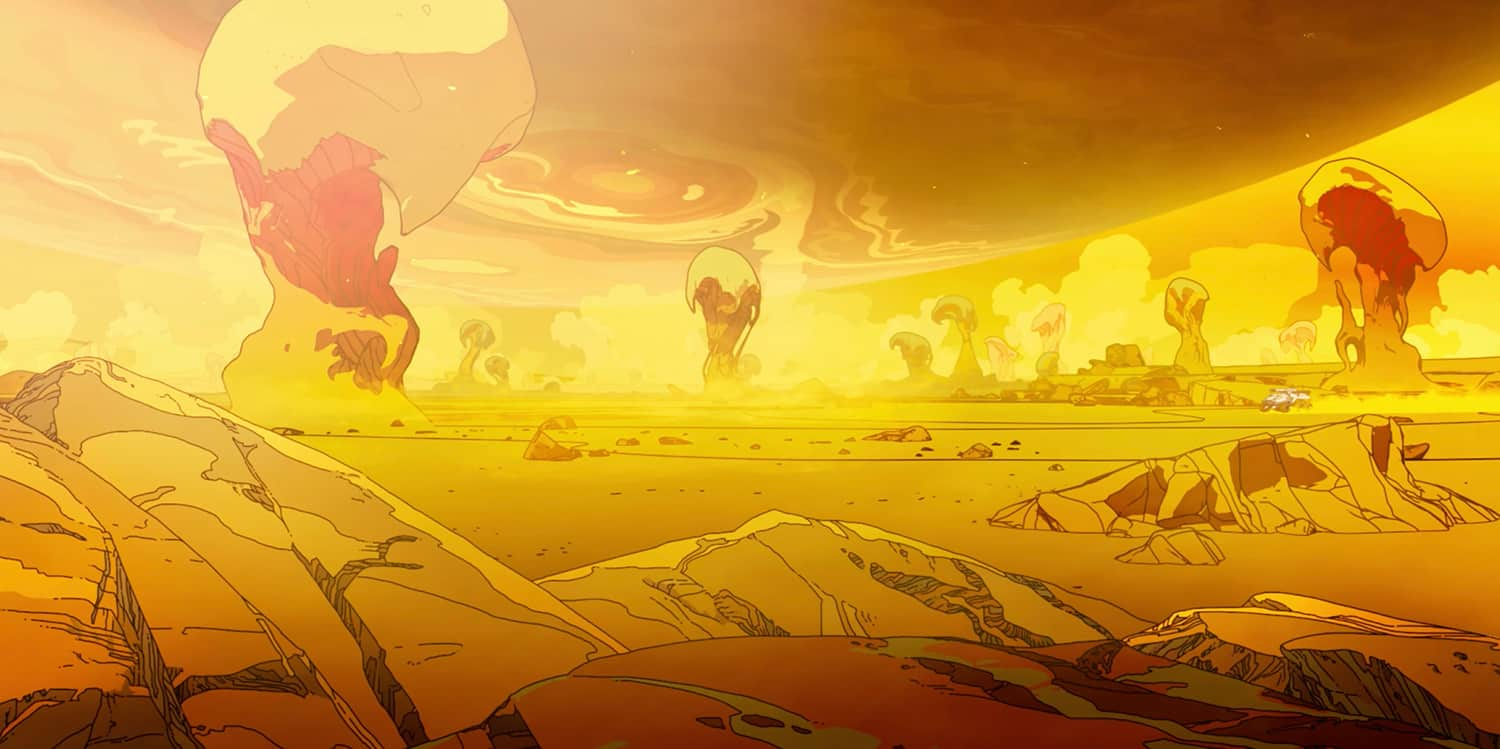
\includegraphics[width=0.6\linewidth]{LoveDeathAndRobotsTVPOTM.jpg}
    \caption[]{Art from a series \emph{Love, Death, and Robots} is the main inspiration for the style.\footnotemark}
\end{figure}

\footnotetext{Episodes \href{https://imdb.com/title/tt9788510/mediaviewer/rm1477017601/?ref_=tt_ov_i}{14} and \href{https://www.artstation.com/artwork/WmkoVJ}{29}, respectively}

\end{document}
